% ---- pg-150 （书页 138） ----

为了确定超过规定容许水平的概率, 需要有辐射量的概率分布. 能否把观测值当作是正态分布呢?

使用计算机来综合处理点对 $(q_{(i)},x_{(i)})$ 以及构造这 Q-Q 图, 示于\hyperref[fig:4.6]{图 4.6}. 由数据作的散点图从整体来看似乎不是正态分布. 图中用圆圈标出的点是离群值——这些值相对于其他观测值太大了.

\begin{mvfigure}
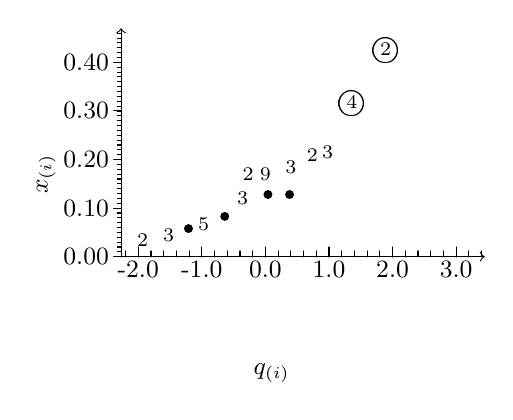
\begin{tikzpicture}[scale=0.95,line join=round,line cap=round]
% 数据坐标 -> cm: x 每单位 0.85cm, y 每单位 6.5cm
\draw[->] (-2.30*0.85,0) -- (3.45*0.85,0);
\draw[->] (-2.27*0.85,0) -- (-2.27*0.85,0.47*6.5);
% x 轴小刻度(每 0.2)与主刻度
\foreach \t in {-2.2,-2.0,...,3.4} {
  \draw (\t*0.85,0) -- (\t*0.85,0.012*6.5);
}
\foreach \t/\lab in {-2/-2.0,-1/-1.0,0/0.0,1/1.0,2/2.0,3/3.0} {
  \draw (\t*0.85,0) -- (\t*0.85,0.020*6.5);
  \node[below,inner sep=1.5pt,font=\small] at (\t*0.85,0) {\lab};
}
% y 轴小刻度(每 0.01)与主刻度
\foreach \t in {0.00,0.01,...,0.46} {
  \draw (-2.27*0.85,\t*6.5) -- (-2.27*0.85-0.05,\t*6.5);
}
\foreach \t/\lab in {0/0.00,0.1/0.10,0.2/0.20,0.3/0.30,0.4/0.40} {
  \draw (-2.27*0.85,\t*6.5) -- (-2.27*0.85-0.10,\t*6.5);
  \node[left,inner sep=1.5pt,font=\small] at (-2.27*0.85-0.10,\t*6.5) {\lab};
}
\node[font=\small,rotate=90] at (-2.27*0.85-1.00,0.17*6.5) {$x_{(i)}$};
\node[font=\small] at (0.1*0.85,-0.24*6.5) {$q_{(i)}$};
% 数据点（同一位置上的点重合为一个点，旁边的整数为点的个数）
\fill (-1.21*0.85,0.058*6.5) circle (1.7pt);
\fill (-0.64*0.85,0.083*6.5) circle (1.7pt);
\fill (0.04*0.85,0.128*6.5) circle (1.7pt);
\fill (0.38*0.85,0.128*6.5) circle (1.7pt);
% 数据点个数标签：\scriptsize + inner sep=1pt，并抬高"2""9"两处避免压点
\node[font=\scriptsize,inner sep=1pt] at (-1.93*0.85,0.033*6.5) {2};
\node[font=\scriptsize,inner sep=1pt] at (-1.52*0.85,0.044*6.5) {3};
\node[font=\scriptsize,inner sep=1pt] at (-0.97*0.85,0.067*6.5) {5};
\node[font=\scriptsize,inner sep=1pt] at (-0.36*0.85,0.120*6.5) {3};
\node[font=\scriptsize,inner sep=1pt] at (-0.27*0.85,0.170*6.5) {2};
\node[font=\scriptsize,inner sep=1pt] at (0.00*0.85,0.170*6.5) {9};
\node[font=\scriptsize,inner sep=1pt] at (0.40*0.85,0.184*6.5) {3};
\node[font=\scriptsize,inner sep=1pt] at (0.74*0.85,0.208*6.5) {2};
\node[font=\scriptsize,inner sep=1pt] at (0.98*0.85,0.214*6.5) {3};
% 离群值
\node[font=\small] at (1.36*0.85,0.310*6.5) {\textcircled{\scriptsize 4}};
\node[font=\small] at (1.89*0.85,0.420*6.5) {\textcircled{\scriptsize 2}};
\end{tikzpicture}
\phantomsection\label{fig:4.6}\mvcap{图 4.6\quad 例 4.10 的辐射量(炉门关闭)数据的 $Q$-$Q$ 图\\
(图中的整数表明在同一位置上的点的个数)}
\end{mvfigure}

对放射量数据, 有些观测值是相等的. 在这情况出现时, 有相同值的那些观测值伴有相同的正态分位数. 这个分位数是用观测值在全都略有不同时所有的分位数的平均值算出的.\hfill$\blacksquare$

Q-Q 图的直线性可以通过计算图中点的相关系数来度量. Q-Q 图的相关系数由下式定义
\phantomsection\label{eq:4-31}
\begin{equation}
r_{Q}=\frac{\sum_{j=1}^{n}(x_{(j)}-\bar{x})(q_{(j)}-\bar{q})}{\sqrt{\sum_{j=1}^{n}(x_{(j)}-\bar{x})^{2}}\sqrt{\sum_{j=1}^{n}(q_{(j)}-\bar{q})^{2}}} \tag{4-31}
\end{equation}
并且可以根据它对正态性进行有力的检验(参见文献[5], [10]和[12]). 形式上, 在显著性水平 $\alpha$ 下, 如果 $r_{Q}$ 降为\hyperref[tab:4.2]{表 4.2} 中适当值之下, 我们拒绝正态性假定.

\begin{mvtable}
\phantomsection\label{tab:4.2}\mvtabcap{表 4.2\quad 对正态性的 $Q$-$Q$ 图相关系数检验的临界点}
\begin{tabular}{cccc}
\toprule
\multirow{2}{*}{样本容量 $n$} & \multicolumn{3}{c}{显著性水平 $\alpha$} \\
\cmidrule(lr){2-4}
 & 0.01 & 0.05 & 0.10 \\
\midrule
5 & 0.829 9 & 0.878 8 & 0.903 2 \\
10 & 0.880 1 & 0.919 8 & 0.935 1 \\
15 & 0.912 6 & 0.938 9 & 0.950 3 \\
20 & 0.926 9 & 0.950 8 & 0.960 4 \\
25 & 0.941 0 & 0.959 1 & 0.966 5 \\
30 & 0.947 9 & 0.965 2 & 0.971 5 \\
35 & 0.953 8 & 0.968 2 & 0.974 0 \\
40 & 0.959 9 & 0.972 6 & 0.977 1 \\
45 & 0.963 2 & 0.974 9 & 0.979 2 \\
\bottomrule
\end{tabular}
\end{mvtable}
